% Taken verbatim from comps Q6

% Typically, when studying local keys computationally, an overlap between modulations, tonicizations, and chords is also observed, and this can be corroborated in the literature that uses local key estimation as means for chord detection. \todo{there are papers that do exactly this}

In music theory, \emph{modulation}, \emph{applied dominants}, and \emph{tonicization} are related (but not interchangeable) terms that describe the change of the musical key throughout the piece. The term \emph{modulation} is at least as old as Jean-Philippe Rameau's \emph{Trait\'e de l'harmonie} \cite{rameau1971treatise}, while the terms \emph{applied dominant} and \emph{tonicization} seem to have emerged from the functional theory of Riemann around the 19th century \cite{gollin2012reception}.

In Music Information Retrieval (MIR), it is common to describe the context in which a key-finding algorithm operates by making use of two terms, namely, \emph{local} and \emph{global} key. A local key is related to the music-theoretical concepts of \emph{modulation}, \emph{applied dominants}, and \emph{tonicization}. However, such relationship is not well-defined. The global key is related with the key of the piece or work, for example, as written in the title of the score. Generally, that relationship is well-defined.

Ideally, the concepts of \emph{modulation}, \emph{applied dominants}, \emph{tonicization}, \emph{local}, and \emph{global} key, are well delimited and the difference (or equivalence) between them is a consensus. In practice, unfortunately, this is not the case. 

This might seem like a minor complication, however, it presents two significant problems for the MIR research community. The first problem is that it affects the evaluation of certain MIR algorithms, which is one of the ways in which the MIR field makes progress. The second problem is that virtually any modern MIR algorithm requires ground-truth data for training, and when the ground-truth data is highly ambiguous, it is not very useful for training new models.

In the following section, a few of the uses of these terms are discussed in the context of music theory and MIR research.

\guide{The terminology in MIR}
MIR, as a research field, has made use of the concepts of modulation, applied dominants, tonicization, local key, and global key, mostly in the design of new algorithms that retrieve such musical information from the input.

Purwins et al., for example, introduced a method for tracking \emph{modulations} in audio signals \cite{purwins2000new}. In order to test their model, they compared the segmentation of their algorithm with an expert annotation of Chopin's Prelude Op. 28 No. 20. In the expert annotation, there are changes of key that happen as quickly as after a quarter note. In the annotation, those changes are marked with parentheses (as tonicizations), however, the model from Purwins et al. does not make a distinction between the two types of annotations. The term \emph{local} key does not appear in the paper either.

In 2014, Pauwels and Martens proposed a system that was both, a local key-finding and chord recognition algorithm \cite{pauwels2014combining}.\footnote{This combination of local key and chords has become increasingly popular in many MIR systems.} In their paper, they discuss the distinction between local and global keys. In their definition, a local key assigns a key label to a time segment of the input and a global key assigns a key to an entire \emph{song}.

Chai and Vercoe designed a model for detecting the change of key \cite{chai2005detection}. In their paper, the term \emph{modulation} means ``a change of key''. They do not make use of the terms tonicization or local key.

Catteau et al. introduced a model for key and chord recognition. Part of their model deals with \emph{modulation}. In their context, a modulation is defined in a similar way than the modulations in the chord sequence experiments by Krumhansl and Kessler \cite{krumhansl1982tracing}, which considered that each chord belonged to a certain key. Catteau et al. also borrowed the chord sequences from Krumhansl and Kessler to test their model.

Izmirli introduced a local key and modulation detection model \cite{izmirli2007localized}. In the paper, he discusses the concepts of tonicization, secondary functions, and modulation: ``\emph{Secondary functions and tonicizations are heard as short deviations from the well-grounded key in which they appear - although the boundary between modulation and tonicization is not clear cut. A modulation unambiguously instigates a shift in the key center}''. Additionally, for Izmirli, modulations and local keys are not the same. The distinction is not explicitly clarified, but he probably considers modulations to be the \emph{changes} of key, while the local keys represent the resulting \emph{regions} in a specific key. His work is one of the few works in MIR that addresses, at least briefly, the terminology regarding musical keys. 

In their work on a local key-finding algorithm \cite{papadopoulos2009local}, Papadopoulos and Peeters adopted a very similar approach as Izmirli \cite{izmirli2007localized}. A modulation is the precise moment when there is a change of key, while a local key is the resulting segmentation of the piece in different keys.

% \begin{figure}[h]
%     \centering
%     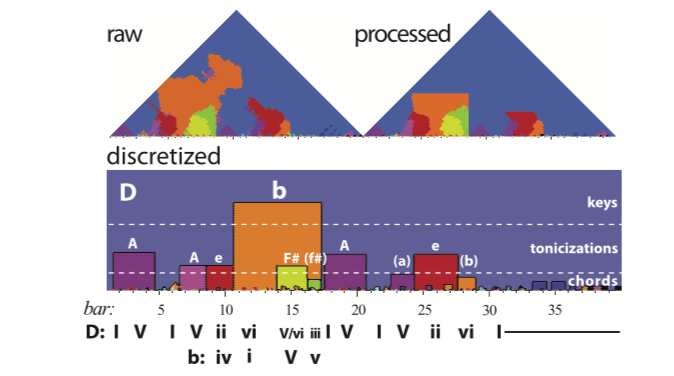
\includegraphics[width=0.7\textwidth]{figures/Q5_1.png}
%     \caption{Visualization of the difference between a modulation and a tonicization, according to Sapp \cite{sapp2011computational}. The horizontal lines in the bottom plot delimit a tonicization from a modulation}
%     \label{fig:Q5_1}
% \end{figure}

Finally, Sapp discussed the possible overlap of the terms modulation and tonicization in music theory and proposes that the difference between a modulation and a tonicization can be observed in his \emph{keyscape} diagrams \cite{sapp2011computational}. This visualization can be seen in Figure \ref{fig:Q5_1}, the dotted horizontal lines \emph{separate} one concept from another. In the paper, Sapp did not include any evaluation that compared whether the annotations from an expert theorist would match the divisions in his \emph{keyscapes} figures. Yet, this is probably the only---quantitative and computationally-applicable---proposal for distinguishing a modulation from a tonicization.


\guide{The terminology in music theory}

In traditional music theory, the terms \emph{local key} and \emph{global key} are virtually non-existent. The issues of ambiguity concern mostly the distinction between tonicization, modulation, and applied dominants.

Regarding this, Kostka and Payne write in their book \cite{kostka2018tonal}: \emph{The line between modulation and tonicization (using secondary functions--V/V and so on) is not clearly defined in tonal music, nor is it meant to be. One listener might find that a very short passage tonicizing a new tonality is enough to make a convincing modulation}.

Holtmeier writes about Hauptmann’s theory and the emergence of applied dominants as a terminology \cite{gollin2012reception}: \emph{In the eyes of its supporters, function theory was predestined ``to demonstrate how superficial are judgments that assert: `Wagner is always modulating!' '' Applied dominants and Hauptmann's concept of the "major-minor key“ allow the theory of functions to interpret harmonically rich progressions within one key without having to invoke modulations. The idea of the applied dominant was the necessary harmonic linking module, so to speak, within a conception of tonality that had distanced itself from a narrow diatonic notion of relations.}

Tchaikovsky does not talk about tonicization \cite{tchaikovsky2005guide}, instead, discusses \emph{transient modulations}. Transient modulations are modulations in which several keys are reached first, temporarily, before arriving to the final key destination.

% \begin{figure}[h]
%     \centering
%     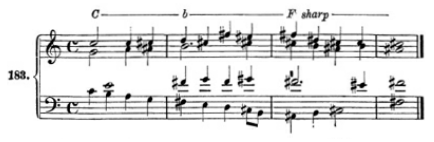
\includegraphics[width=0.7\textwidth]{figures/Q6_2.png}
%     \caption{Example of a \emph{transient modulation} as it appears in Tchaikovsky's manual of harmony.}
%     \label{fig:Q6_2}
% \end{figure}

For Rameau \cite{rameau1971treatise}, the concept of a modulation, rather than a change of key, seems to refer to a key region (similar to what Izmirli and Papadopoulos would consider a local key). This is most clear in his seventh rule for passing from one key to another: \emph{After having passed through several other keys, we must modulate in this principal key for a little longer towards the end than at the beginning.} The fact that one may ``modulate for a little longer'' in a given key, is an uncommon idea in later music theories. In this sense, Rameau's modulation is, in some way, more compatible with modern local key-finding algorithms.





% \guide{What is a modulation?}

% A shift between a previously established key and a new perceived key
% A change in the distribution of pitch classes of the current scale
% A perfect authentic cadence in a different key than the main key(?)


% \guide{What is a tonicization?}
% A sudden reinterpretation of the tonal context for a specific chord or short chord sequence
% A deceptive modulation, which abruptly comes back to the original key
% A modulation that happens on a local scale, without major implications on the length of a piece
% The term tonicization was introduced later in music history, mostly to distinguish meaningless modulations from “real” modulations



% \guide{Differentiating a modulation from a tonicization}
% Most people who study these concepts quantitatively agrees that these concepts differ only in their scale, but represent the same phenomenon
% People who disagree with the two concepts being different only in their length will typically do it on the basis of structural constraints (or rules) that apply to modulations for being modulations and do not apply to tonicizations
% This sort of disagreement lies within what Temperley calls the “distributional” and “structural” views of computational music analysis


% \guide{Dealing with keys in computational studies}

% Computationally, researchers have usually characterized this phenomenon (different musical keys within a piece) with the umbrella term, local keys, which differs with the key of the entire piece, that is, the global key
% Local keys refer to keys within a sequence of music
% Global keys refer to the principal (or main, or first and last key) of a sequence of music
% This is also problematic and controversial
 
 
%  \guide{On the unambiguous determination of local and global keys}
% Whether we are referring to a symbolic or audio representation of music, musical inputs such as the ones received by a key-finding algorithm are typically sequential. 

% In symbolic representations, the units of the input sequences can take the form of individual notes, onset slices with one or more notes, measures, pitch-class vectors, or other units.

% In audio representations, the units of the input sequences usually take the form of samples of a waveform or a spectral representation.

% If we want to differentiate the terms local and global key, one way of doing it is by providing a \emph{local} key label for each element of the sequence that is received by the algorithm. For example, if the symbolic music file received by a key-finding algorithm consists of 4,000 notes, the local keys could consist of 4,000 key labels, associated with each of the notes in the input, and a global key that explains the overall key of the 4,000 notes.

% In the image domain, this is a very common procedure known as image segmentation. In image segmentation tasks, usually one class is assigned to every pixel in the image. This ensures that 

% A sequence of music is a sequence of musical input nodes
% If we talk about symbolic: the sequence is a sequence of notes and rest symbols
% IF we talk about audio: The sequence is a sequence of audio frames and their FFT output
% How long is that sequence? As long as it is relevant for a particular analysis
% A local key is a key that explains the key of the minimum node of that sequence
% A global key is a key that explains the key of the sequence itself
 
 

% \guide{The length of a piece}
% Easiest solution, describes a single movement
% Single movements are not always explained by a single key
% This issue can suffer of similar contradictions as modulations/tonicizations